\chapter{Related Work}
\label{related_work}
The related work chapter is divided into three sections, KGEs, rule mining and approaches combining the two methods. For perspective, it is worth noting that KGEs and rule mining are two KG completion methods at the opposite ends of the rule vs predictive spectrum, depicted in figure \ref{scale}. On the left hand side there are methods that prioritize rule extraction over triple prediction. As one moves from the left gradually to the right there are methods that to an increasing degree prioritize triple prediction over rule extractions. KGEs are furthest to the right on this scale, while rule mining methods furthest to the left. It is these two groups that have been used in the thesis and so works within these areas will be the focus of the related works chapter. This figure can however serve as a reminder that there are many other methods in the grey area between the two extremes. 

\begin{figure}[htbp]
\centering
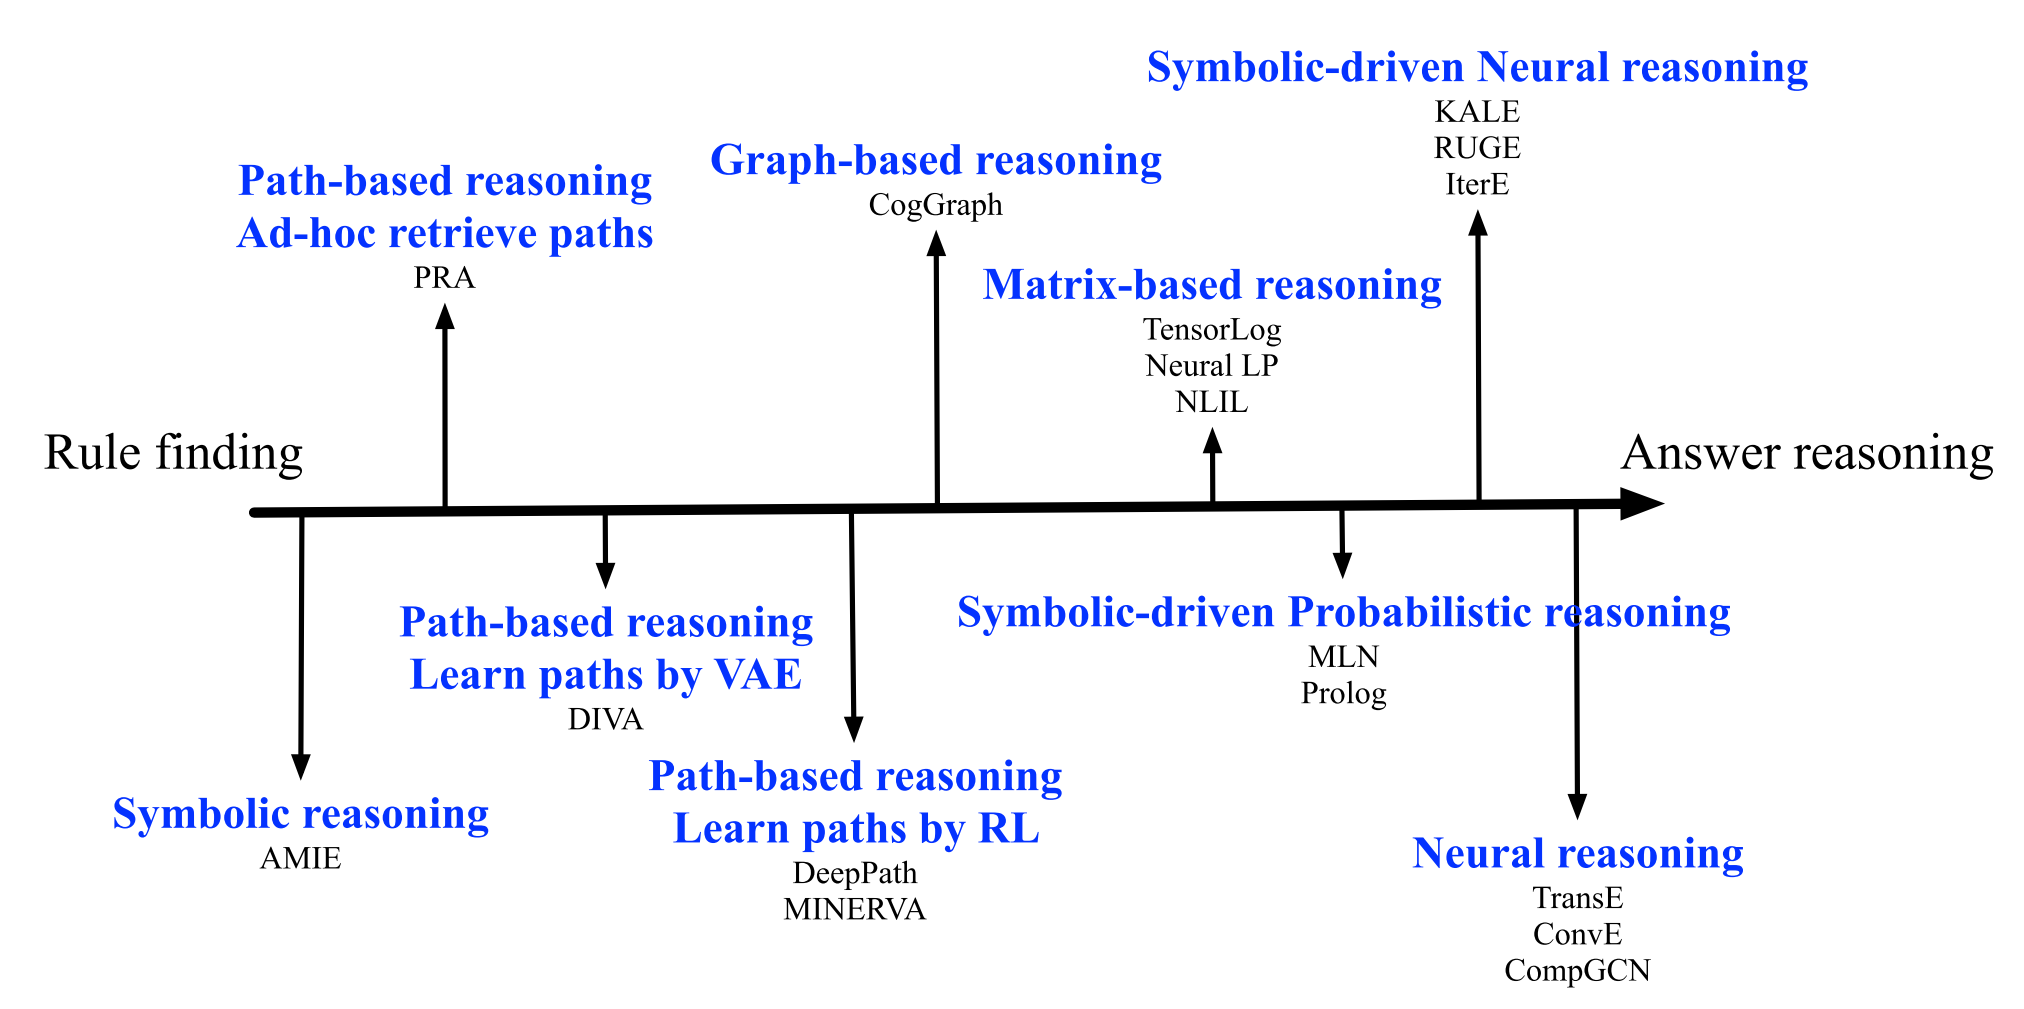
\includegraphics[width=1\linewidth]{figures/related_works/Screenshot.png}
\caption{Knowledge graph completion techniques arranged by the degree to which rule finding or triple prediction is the focus. Source:  https://www.sciencedirect.com/science/article/pii/S2666651021000061   TODO: make own fig}
\label{scale}
\end{figure}

\section{Knowledge graph embeddings}
A wide range of statistical based relational learning techniques have been proposed for KG completion \cite{nickel2015review}. Out of these methods, vector space embedding approaches is one of the most successful due to their performance and scalability. One of the main problems with vector space embeddings, as with many other statistical machine learning methods, is that the results are not explainable \cite{bonatti2019knowledge}. Rule based approaches alleviate this problem to some degree. Early works within vector space embeddings include TransE \cite{TransE} and DistMult \cite{yang2014embedding}, which employ simple vector space operations for link prediction. These simple models are capable of handling large scale knowledge graphs, but this is often at the cost of expressiveness \cite{dettmers2018convolutional}. There have been many attempts at increasing expressiveness while maintaining simplicity, such as SimplE \cite{SimplE}, HolE \cite{holE}, and RotatE \cite{rotatE}. A more direct approach for increasing expressiveness is the employment of deep neural networks. This has been done using multi-layer perceptrons \cite{dong2014knowledge}, semantic matching energy networks \cite{bordes2014semantic} and neural tensor networks \cite{socher2013reasoning}. It has however been shown that these approaches have more parameters and are prone to overfit \cite{nickel2015review}. Improving upon this, there have been many recent approaches using convolutional neural networks \cite{dettmers2018convolutional, nguyen2017novel, jiang2019adaptive, jiang2021kernel} .


\section{Rule mining}
Traditional rule mining methods find rules of quality by statistically evaluating support and confidence on candidate rules. AMIE and it's successors are part of this group, and have for a while been considered at the forefront of both scalability and performance when it comes to mining first-order Horn rules from knowledge graphs. Exact statistical evaluation of rules is expensive, and so there have been approaches adopting embedding methods to score rules \cite{yang2014embedding, omran2018scalable, omran2019embedding}. The rule miner AnyBURL uses rule generation methods different from AMIE, where rules are generated by sampling paths in the KG \cite{meilicke2020reinforced}. These rules are evaluated with the same metrics, but scores are approximated based on sampling in contrast to the exact evaluation done in AMIE3. AnyBURL used reinforcement learning to improve their sampling of paths, leading to higher quality rules being found earlier in the search. A more recent approach to rule mining with reinforcement learning takes advantage of embedding information to achieve better performance and allows scalable mining of long rules \cite{chen2022rule}. This method outperforms AMIE+, and the authors point out that the many optimizations made to AMIE+ (resulting in AMIE3) could be applied to any top-down rule mining methods, including theirs. Top-down in this context means beginning the search with the most general rules and then expanding on them, essentially performing a breadth-first search in the space of possible rules. The bottom-up approach on the other hand works from the data, starting with very specific rules and then generalizing them.

A KG completion family similar to rule mining is path-based reasoning methods. One of the first of these was the \textit{path ranking algorithm} (PRA) \cite{lao2011random}. This approach trains a binary classifier for each relation $r$ in the KG, that given two entities $h$ and $t$ determines if they are connected via a relation $r$. Path ranking algorithms struggle with sparseness in KGs \cite{ma2019elpkg}, and so there have been attempts at combining PRAs and embedding methods. An example of this is PTransE, which considers relation paths with multiple steps, and uses embedding methods similar to TransE to represent these paths \cite{lin2015modeling}.  % does this really need to be here?


\section{Approached combining KGE and rule mining}
When it comes to combining the rule based and embedding based approach there seem to be two main ideas. The first idea is to tightly integrate the two approaches. An example of this is KALE \cite{KALE}, which initially learns rules from a TransE embedding and thereafter retrains the embeddings on a joint model for rules and triples, resulting in a unified framework. Based on KALE, Guo et al. proposed RUGE \cite{RUGE}, which learns entity and relation embeddings through iterative guidance from soft rules. The soft rules are queried to obtain soft labels for unlabeled triples, and these newly labeled triples are then used to update the embedding model. It has however been noted that these systems generally do not allow for rules that contain constants \cite{meilicke2021naive}. KALE and RUGE infer rules once at the beginning of the process, therefore the embedding can benefit from information in the rules, but the rules are never improved upon with the embedding. IterE \cite{zhang2019iteratively} addresses this issue and also infers new rules based on the updated embedding. The update of rules and embeddings is done iteratively, and the rules are given a score based on the embedding of the relations that are included in the rules.

The second idea proposes to combine the rule based and embedding models into an ensemble. An ensemble is a machine learning method that uses multiple models to obtain a better prediction than one would with a single model. This is often done by allowing models to ``vote" upon a prediction. The ensemble approach has been studied by Wang et al. \cite{wang2018multi} and was the focus of the experimental study by Meillicke et al. \cite{ensemble} mentioned in the introduction. The authors recently extended this study with a more up-to date analysis, where they explain ``\textit{why a naive way to combine symbolic and latent knowledge graph completion techniques works surprisingly well}" \cite{meilicke2021naive}. The work in this thesis combines rule based and embedding models in a different manner, where the information gained by one model is passed on to the next in the form of an extended, or more ``complete", KG. While the first model influences the outcome of the next, it does not play a direct role in the final outcome, in this case the outcome being the rules mined from the KG.

